\documentclass[10pt,a4paper]{article}
\let\vec\vec
\usepackage[utf8]{inputenc}
\usepackage{newtxtext,newtxmath}
\usepackage{amsmath,amssymb}
\usepackage{natbib}
\textwidth 440pt
\textheight 680pt
\voffset -50pt
\parindent 0pt
\oddsidemargin 20pt
\usepackage{url,hyperref}
\usepackage{graphicx}
\usepackage{subfig}

% journal shorthand
\newcommand\aj{AJ}                   	% Astronomical Journal (the)
\newcommand\mnras{MNRAS}    % Monthly Notices of the Royal Astronomical Society
\newcommand\aap{A\&A}              % Astronomy and Astrophysics
\newcommand\apjs{ApJS}               % Astrophysical Journal, Supplement
\newcommand\apj{ApJ}                 % Astrophysical Journal
\newcommand\nat{Nature}              % Nature
\newcommand\araa{ARA\&A}             % Annual Review of Astronomy and Astrophysics
\newcommand\aapr{A\&ARv}             % Astronomy and Astrophysics Review (the)
\newcommand\apjl{ApJL}
\newcommand\pasp{PASP}
\newcommand\rmxaa{Rev. Mex. Astron. Astrofis.}
\newcommand\procspie{Proc.~SPIE}

\begin{document}

\title{{\bf DRAFT 2:} section 1.3 - Baryon cycles in the circumgalactic medium}
\author{S. Kolwa}
\maketitle

% To improve on this:
% Maybe go into more detail about the physics underlying the various tracers (for Schaile and Biebel - the physicists)
% Motivate why these tracers are important - what do they tell us about the thermodynamics, ionisation state etc

\section{Baryon cycles in the circumgalactic medium} 
\subsection{The circumgalactic medium} 
The circumgalactic medium (CGM) is commonly defined as the region of gas surrounding a galaxy that extends out to distance scales of hundreds of kpc from its nucleus. The CGM thus extends well beyond the intersteller medium (ISM) of a galaxy which may have scale sizes approximately within the range of $\sim$10-20 kpc. Then further beyond even the CGM, is the intergalactic medium (IGM) which can extends out to tens of Mpc around a gravitationally bound group of interacting galaxies. Thus, the CGM defines the gas that is located  somewhere between the ISM and IGM and acts as an interface for gas processes (inflow and outflow for instance) between ISM and IGM. The approximate diametric size of a typical CGM is indicated in the now ubiquitous diagram shown in Fig \ref{fig:CGM-Tumlinson2017} from a review by \citet{tumlinson2017}. This illustration provides examples of physical processes associated with gas from the IGM, CGM and ISM that have either been observed or predicted by hydrodynamic simulations may occur. In reality, these gastrophysical processes are complex to model and, in some respects, difficult to observe due to uncertainties and observing limits of current observing facilities. 

\begin{figure}[!ht]
 \centering
 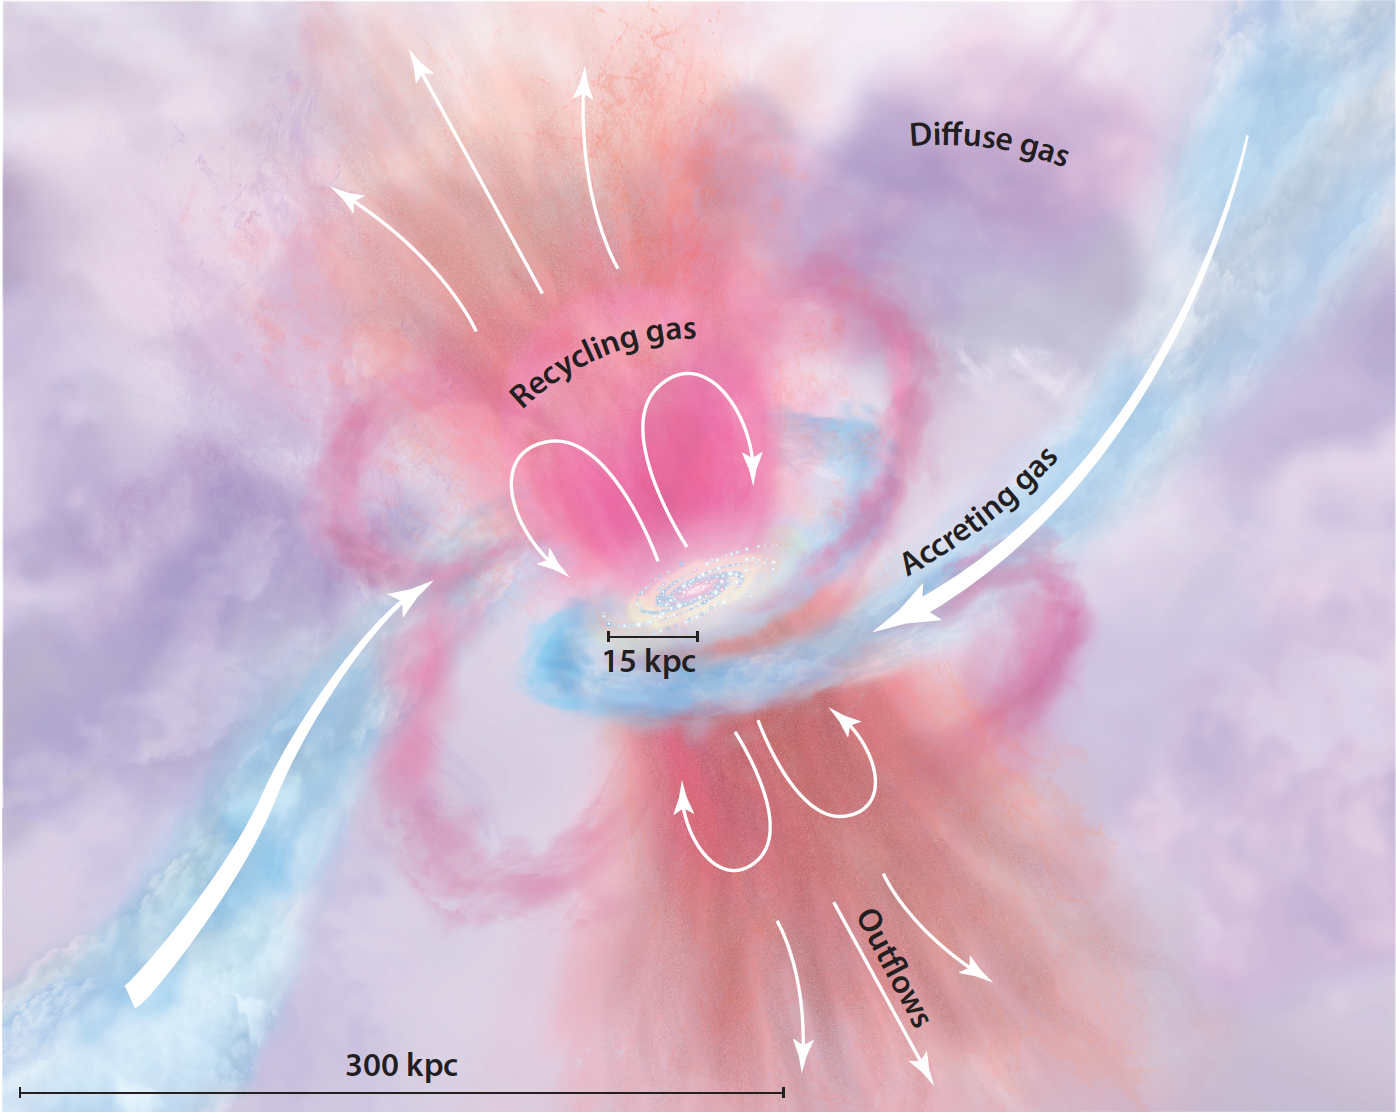
\includegraphics[width=0.8\textwidth]{plots_chp1/CGM_Tumlinson_2017.png}
 \caption[A general view of a galaxy's circumgalactic medium (CGM)]{An idealised illustration of the circumgalactic medium offered by \citet{tumlinson2017} of a galaxy which comprises interstellar medium as well as reservoirs of gas extending out to $\sim$100 kpc from a galaxy's nucleus. }
 \label{fig:CGM-Tumlinson2017}
\end{figure}

The processes and features referred to in Fig. \ref{fig:CGM-Tumlinson2017} are (a) the inflow or accretion of pristine gas from the IGM (b) outflows of gas that may be driven by either stellar and/or AGN feedback events (c) infall of metal-rich gas that has been expelled from the galaxy at velocities $\varv < \varv_{esc.}$ (below the escape velocity) and (d) diffuse extensions of low surface-brightness gas. Provided that the cold molecular gas that fuels star-formation is affected by one of or a combination of these mechanisms, the flow of baryons - gas as well as metals or dust - into and out of the CGM plays a very significant role in the evolutionary path which a galaxy will follow. 

The concept of a CGM only emerged rather recently (in the last ten odd years) within the astronomy lexicon. During this time, both observations and simulations which have improved over the years with the development of new instruments on telescopes and faster computing have been invoked to study the CGM in greater detail. Observationally, some of the main methods for studying the CGM are (a) detecting absorption lines in spectra along a transverse-line in the projected plane of a galaxy (b) mapping out line-emission (c) stacking spectra from faint sources (d) detecting line emission and absorption ``down-the-barrel" or along the line-of-sight and (e) simulating and modelling CGM processes using hydrodynamical simulations and semi-analytic models \citep{tumlinson2017}. I offer a brief explanation of each of these methods and examples from the literature of their usage, here: 

(a) The absorbing gas within the CGM of a galaxy, when viewed against a background quasar, is defined by several  parameters. The first of these is column density which is simply the number of absorbing ions or atoms per unit area along a sightline), Doppler widths given by the $b$ parameter which is defined as $b^2 = 2kT/m + b_{nth}$ in which $k$ Boltzmann constant, $T$ the temperature of the gas medium, and $m$ is the gas particle mass. An additional factor of $b_{nth}$ is added to the Doppler width to account for intrinsic broadening of an emission line resulting from turbulence in the gas. The redshift by fitting Voigt profiles to continuum-corrected absorption lines in nearby galaxies \citep[e.g.][]{Lehner2015,Bowen2016} and more distant lensed quasars \citep[][]{RauchHaehnelt2011, Rubin2015}. 

(b) Additionally, emission line maps of radiation from CGM have been made with the use of deep narrow-band imaging \citep{Prescott2015,Arrigoni-Battaia2016}, integral field unit (IFU) spectroscopes/instruments such as the Keck Cosmic Web Imager (KWCI) as seen in \citet{Cai2018} as well as on the Very Large Telescope (VLT) with Multi-unit Spectroscopic Explorer (MUSE) which provide a spectrum for every pixel in the instrument's field of view \citep[e.g.][]{Cantalupo2014}. 

(c) Stacking spectra is gainful for detecting weak or faint absorption through the co-addition of hundreds to thousands of spectra from large surveys. (d) Emission and absorption detected ``down-the-barrel" of the light-sources using spectroscopy. This method relies on line emission to be produced by starlight and possibly also an AGN within a galaxy. This emission serves as a background source without which constraints on the absorbing gas in front of the emission would not be possible. This way of detecting CGM gas properties is commonly adopted when observers seek direct evidence of inflowing and outflowing gas by tracing where redshifted and blueshifted emission components occur in line-of-sight velocity \citep[][]{Steidel2010,Heckman2015}. (e) Simulations of a galaxy CGM's temperature, metallicity, density have been and continue to be an essential way of grappling the effects of baryon flows over cosmological time-scales as they offer a continuous view instead of snapshots in time which are obtained from the observations \citep[][]{SomervilleDave2015}.

%phases of the CGM
Another important aspect of the CGM is that it is multiphase comprising ionised, molecular and neutral gas complexes. Hydrodynamic simulations such as those of Fig. \ref{fig:phase-diagram-gas-Torrey2019} shown in \citet{Torrey2019} which illustrate the expected baryon phases within the gravitationally bound gas halo at $z=0$ as a function of temperature and density. Hot diffuse gas with $\log{(T/K)} \gtrsim 7$ are predicted by such simulations and have also been observed in soft X-ray emission \citep{AndersonBregman2010}. The warm, ionised gas medium has temperature approximately within the range of $\log{(T/K)} \simeq 4.5 - 6$ and the cooler ionised gas has temperatures of $\log{(T/K)} \simeq 4.$ Conclusions about the temperatures of ionised gas can be drawn from photoionisation equilbrium models (PIE). PIE models can be formed in spectral synthesis modelling code such as {\it Cloudy} \citep{Ferland2013}. 

\begin{figure}
 \centering
 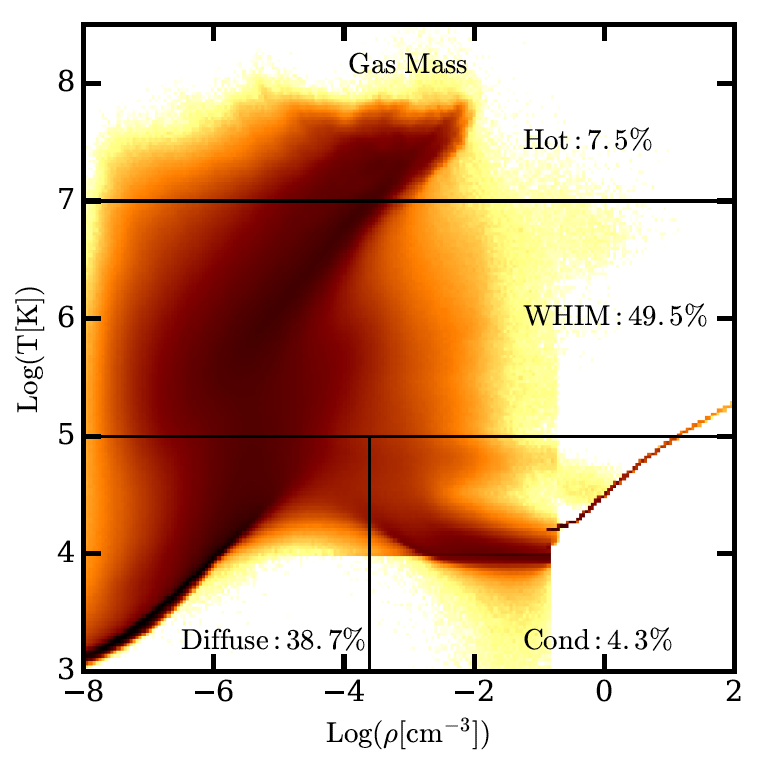
\includegraphics[width=0.7\columnwidth]{plots_chp1/Phase_diag_Torrey2019}
 \caption[Phase diagram of simulated gas-mass distribution at $z=0$]{Phase diagram of gas-mass distribution at $z=0.$ The boundaries between the different gas phases are given along with the fraction of gas phase to the total gas budget. The gas phases are a hot ($\log{(T/K)} > 7$), warm-hot intergalactic medium (WHIM; $5 < \log{(T/K)} < 7$), diffuse ($\rho < 1000\rho_{\rm c}\Omega_{\rm c}$, $\log{(T/K)} < 5$) and condensed gas ($\rho > 1000\rho_{\rm c}\Omega_{\rm c}$, $\log{(T/K)} < 5$) masses which were coined by \citet{Dave2001} and \citet{Haider2016}.}
 \label{fig:phase-diagram-gas-Torrey2019}
\end{figure}

One of the major problems facing CGM studies, however, is that of missing baryons. CGM masses of low to high luminosity galaxies are under-predicted the cosmological baryon to mass density ratio $\Omega_b/\Omega_m=0.16$ constrained by observations by the Planck Mission \citet{Planck2016}. Measurements of galaxy halo masses have indicated that the total mass of baryons is much lower than what is predicted by the $\Lambda$CDM (cold dark matter) cosmology model. In other words, $M_{\rm b} \ll (\Omega_b/\Omega_m)M_h$ where $M_b$ is the total baryon mass, and $M_{\rm h}$ the halo mass. An example of this is illustrated in Fig. \ref{fig:CGM-baryon-budget-Tumlinson2017} where the surface gas densities of multiple gas phases and dust when added do not account for the gas surface density predicted by $\Lambda$CDM cosmology. Many galaxies appear to be missing up to $80\%$ of their baryons implying that the majority of baryons in the CGM are currently undetected. Some have suggested that the missing baryons are in diffuse, hot halo gas that future missions such as the X-ray observatories {\it eRosita} and {\it Athena} \citep{Barret2016} will provide adequate data for addressing. 

\begin{figure}
 \centering
 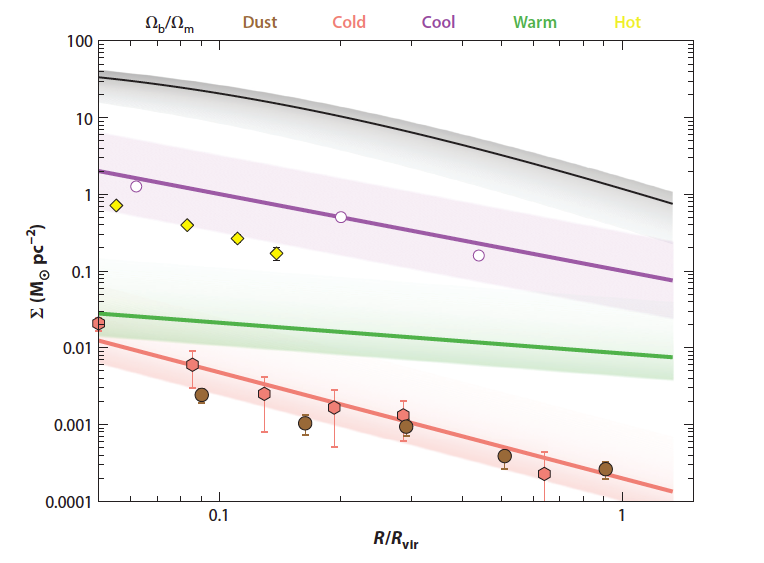
\includegraphics[width=0.8\textwidth]{plots_chp1/CGM_missing_baryons_Tumlinson_2017}
 \caption[CGM mass surface-density profiles of multi-phase components]{Synthesis of CGM mass surface-density profiles of multi-phase components compared to the Navarro-Frenk-White (NFW) profile (black) prediction scaled by $\Omega_b/\Omega_m$ for a dark-matter mass of $M_{\rm DM}/\rm{M}_\odot = 2\times10^{12}.$ The density profiles are for cold gas (salmon) from \citet{ZhuMenard2013a}, cool gas (purple) from \citet{Werk2014}, warm gas (green) traced by OVI ions \citep{Tumlinson2011,Peeples2014}, hot X-ray emitting gas (yellow) \citep{Anderson2016} and dust (brown) \citep{Menard2010}. }
 \label{fig:CGM-baryon-budget-Tumlinson2017}
\end{figure}

I turn my focus to the CGMs of radio galaxies because they are the main focus of this thesis and we can look beyond the ISM, observationally and attempt to find direct evidence of kinetic feedback within their CGMs - provided the observations are of sufficient quality. The CGMs of radio galaxies such as those the HzRGs by the USS method are important because accretion of gas onto the supermassive blackholes of these galaxies leads to tremendous bursts of energy being deposited throughout the extended halo of the galaxy (to distances of $\sim$100 kpc). We can thus observe the effects of the AGN on the galaxy halo through heating, compression, excitation and ionisation of the extended gas medium by way of the radiation and jets produced by the AGN. Tracing the kinematics, state and phases of the CGM in HzRGs is important for understanding the way radio-mode AGN feedback operates. 

\subsection{The CGMs of high redshift radio galaxies} 
Observing the kinematics, morphology and state of the bound gas (haloes) around radio galaxies is pivotal to understanding how the mechanical power of the radio jets plays a role in moderating the galaxy's gas supply. Thankfully, evidence for jet-gas interactions within the gaseous haloes of radio galaxies are plentiful. One of the most effective ways to probe kinematically perturbed gas within the haloes of HzRGs is from the line-width measures, particularly the lines that trace the warm, ionised gaseous medium. Most HzRGs are surrounded by giant complexes of ionised gas traced primarily by Ly$\alpha$ emission nebulae \citep{mccarthy1990a,Reuland2003b}. The Ly$\alpha$ nebulae of HzRGs are known to extend out to to diameters of up to $d \lesssim 200$ kpc. 

\begin{figure}[!ht]
 \centering
 \subfloat[]{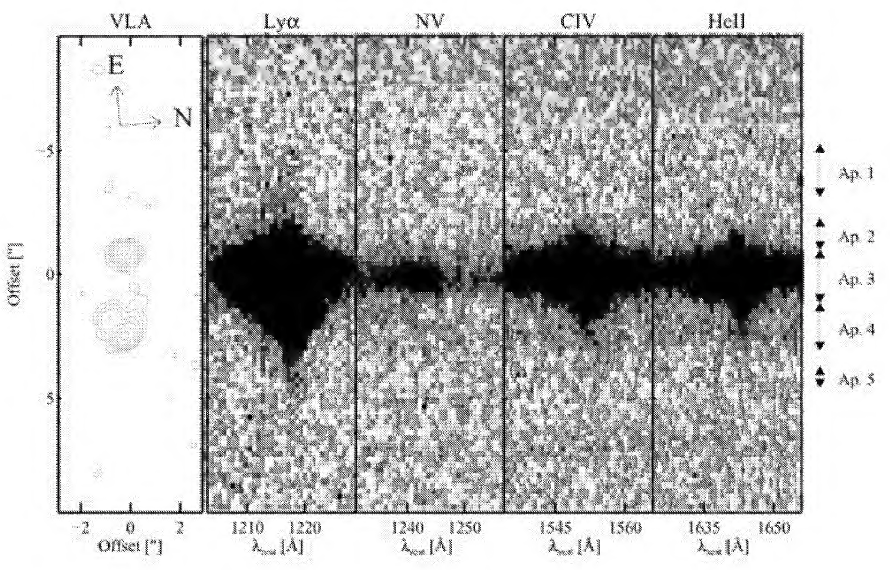
\includegraphics[width=0.7\textwidth]{plots_chp1/pos_velocity_Villar_Martin2003.png}}\\
 \subfloat[]{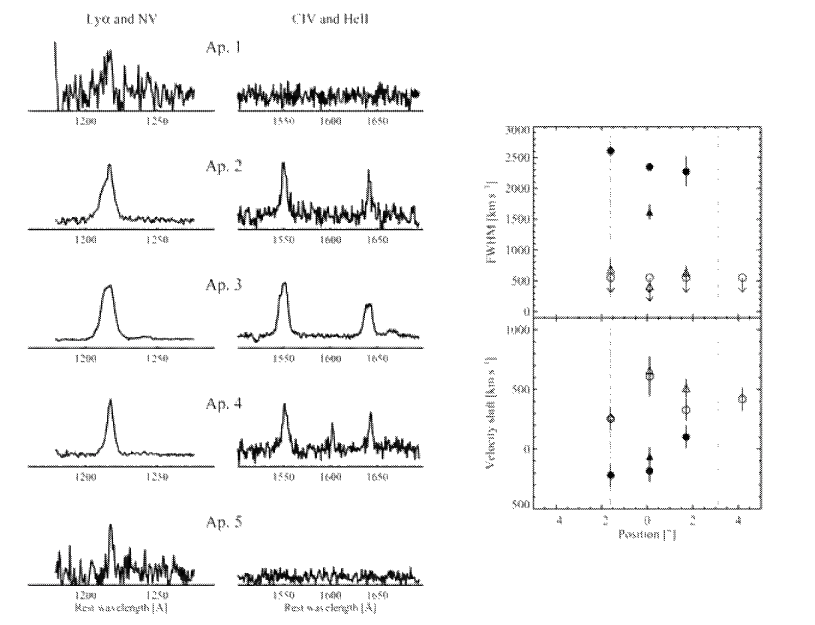
\includegraphics[width=0.7\textwidth]{plots_chp1/spectra_FWHM_vel_shift_Villar_Martin2003.png}}
     \caption[Keck 2D and 1D spectra from \citet{villar-martin2003}]{Panel a: VLA radio map with offsets that are spatially aligned with Keck 2D spectra (position-velocity diagrams) for Ly$\alpha$ $\lambda$1216, NV $\lambda$1238, CIV $\lambda$1550 and HeII $\lambda1640.$ Panel b: Spatially integrated spectra from the apertures labelled in panel a (left). The FWHM and velocity offsets relative to HeII which marks the zero-velocity centroid. The symbols represented are circles for Ly$\alpha,$ and triangles for HeII; filled symbols for broad components and non-filled symbols for narrow kinematic components of an emission line \citep{villar-martin2003}.} 
 \label{fig:kinematics-ionised-Villar_Martin2003}
\end{figure}

\begin{figure}[!ht]
 \centering
 \subfloat[]{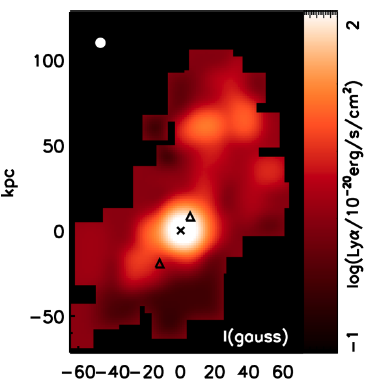
\includegraphics[width=0.5\columnwidth]{plots_chp1/Ly_alpha_intensity_Swinbank2015}}\\
 \subfloat[]{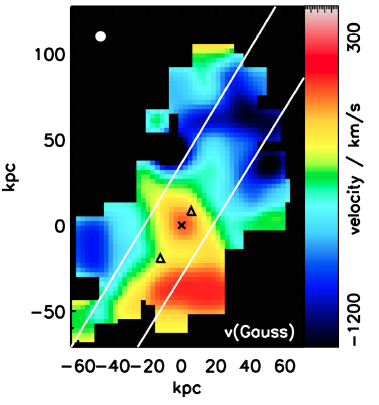
\includegraphics[width=0.5\columnwidth]{plots_chp1/vel_map_Swinbank2015}}
 \caption[Intensity and velocity map from \citet{swinbank2015}]{Panel a: An intensity map of the underlying Ly$\alpha$ emission profile (modelled by a Gaussian). Panel b: Velocity map of the Gaussian emission profile from panel a. The nucleus is shown as a cross and the radio hotspots as triangles. The white lines represent the orientation of the slit along which the velocity shear and HI column density profiles are measured from a 9-h integration on the VLT with the integral field unit (IFU) spectrograph MUSE (Multi-unit Spectroscopic Explorer) \citet{swinbank2015}.}
 \label{fig:TNJ1338-Swinbank2015}
\end{figure}

%Warm, ionised gas medium
In the rest-frame UV spectral regime spanning ($1200 - 1800~\text{\AA}$), the ionised gas medium engulfing a galaxy is probed by rest-UV lines, the most pervasive of which is the hydrogen Lyman-alpha line (HI Ly$\alpha$) at $1215.57~\text{\AA}$. Some of the common lines detected from HzRGs are shown by the composite spectrum of \citet{McCarthy1993} formed by combining observations of several $0.1 < z < 3$ galaxies (see Fig. \ref{fig:comp_spec_RGs}. These lines, when emmissive, trace the warm gas regions at temperatures of, $T_{\rm{e}} \sim 10^{4}-10^{5}$ K, particle densities of $n_{\rm{e}} \sim 10^{0.5} - 10^{1.5} \rm cm^{-3}$ which is gleaned from emission line diagnostics \citep{OsterbrockFerland2006}. In low density regions, forbidden line are also detected. Later observations with improved equipment showed that emission line haloes spanning up to $\sim200 \rm kpc$ are a common feature of HzRGs \citep{Reuland2003a}. 

\begin{figure}
\centering
  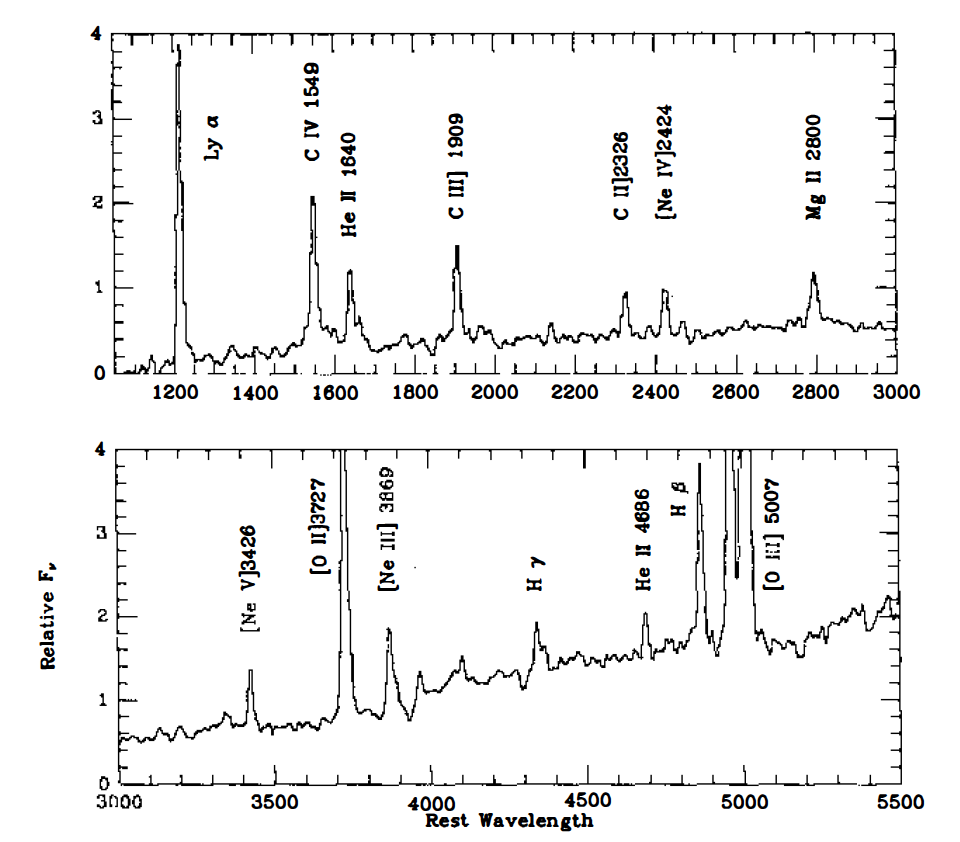
\includegraphics[width=0.65\textwidth]{plots_chp1/UV_spectrum_McCarthy2003}
  \caption[Composite radio galaxy spectrum from galaxies at $0.1 < z < 3$]{Composite radio galaxy spectrum obtained from galaxies at $0.1 < z < 3$ comprising data from the telescopes, Kitt Peak 4-m, Lick 3-m, and Palomar 5-m with $2.5'' \times 3"$ apertures. }
  \label{fig:comp_spec_RGs}
\end{figure}

The high surface-brightness regions within the extended haloes are characterised by by turbulent kinematics where spectral lines that trace the ionised gas are broadened to widths of $\rm FWHM \gtrsim 1000$ km s$^{-1}$ and powered to luminosities of up to $\rm 10^{44}~erg~s^{-1}$ \citep{mccarthy1996,villar-martin1999a}. In addition to being high energetics and turbulent gas motions, these inner halo regions also have clumpy morphologies when observed under UV/optical imaging from instruments such as the {\it Hubble Space Telescope} (HST) Wide-field Planetary Camera 2 (WFPC2) and {\it Keck} long-slit spectroscopy \citep{humphrey2006,Villar-Martin2006}. Further away from the nucleus, HzRG haloes have more quiescent kinematics with line widths of the order, $\rm FWHM \simeq 100$ km s$^{-1}$ and smoother UV/optical morphologies consistent with gas that is dynamically relaxed as is described in \citet{villar-martin2003} (Fig. \ref{fig:kinematics-ionised-Villar_Martin2003}). 

Recent observations of HzRGs using IFU spectroscopy have confirmed much of what has been known of the kinematics and morphology of their gaseous haloes. MUSE, which has a sufficiently low sensitivity to probe extended diffuse emission in the optical, has been important in bringing about a spatially resolved view of emission from ionised gas in the extended gas haloes of distant radio galaxies. In \citet{swinbank2015}, narrow-band imaging of the $z=4.1$ radio galaxy (TN J1338-1942) reveals its colossal $\sim$150 kpc diameter Ly$\alpha$ nebula. Mapping out the velocity in this source showed that it has a velocity gradient of up to $\sim$1000 km s$^{-1}$ along the extent of its nebula (as shown in Fig. \ref{fig:TNJ1338-Swinbank2015}). MUSE IFU data was also important in showing the morphologies of emission in the galaxy MRC 0943-242 from Ly$\alpha$ as well as other rest-UV lines such as HeII $\lambda1640$, CIV $\lambda1550$ and CIII] $\lambda1907$ and CII] $\lambda2326$ and a velocity gradient across the halo \citep{Gullberg2016a,Silva2018}. 

The neutral phase of the gas haloes of HzRGs can be probed via Ly$\alpha$ absorption. The absorption troughs seen against the emission in Ly$\alpha$ are considered to originate from neutral hydrogen located in front of the extended emission line regions along the line-of-sight \citep{rottgering1995,vanojik1997}. The neutral gas which when fit with Voigt profiles is found to have HI column densities of $\log{ (\rm N_{HI} /cm^{-2}) } \simeq 18-20$ may be associated with the galaxy (located within its ISM or CGM) or be a part of intervening absorption and therefore part of the Ly$\alpha$ forest with $\log{ (\rm N_{HI} /cm^{-2}) } \simeq 13-15$  \citep{wilman2004}. In addition to Ly$\alpha,$ other resonant lines such as CIV $\lambda1550,$ NV $\lambda1238$ and SiIV $\lambda1402.$

The molecular phase of HzRG haloes can be traced via the various fine-structure transitions of the carbon monoxide molecule. CO emission lines trace molecular hydrogen due to collision excitation of $^12$CO by the H$_2$ molecule which result in emission from the rotational transitions $J=1\rightarrow0, 2\rightarrow1, 3\rightarrow2, 4\rightarrow3$ and $5\rightarrow4$ \citep{SolomonvandenBout2005}. Several HzRGs have been detected in these CO transitions \citep{Scoville1997,Alloin2000,deBreuck2003a,Papadopoulos2000,
Greve2004,deBreuck2005,Klamer2005,Ivison2008,Emonts2014,emonts2015,Gullberg2016b}. The observations that provided these results were obtain from mm/sub-mm interferometry on instruments such as Australia Telescope Compact Array (ATCA), Owens Valley Radio Observatory (OVRO), IRAM Plateau de Bure Interferometer, Atacama Pathfinder Experiment (APEX) and the Atacama Large Milimetre/sub-milimetre Array (ALMA) among others. 

\citet{PapadopoulosGreve2004} were first to demonstrate that emission from the fine-structure transitions in atomic carbon can trace H$_2$ in low-redshift ($z\sim0.018 - 0.043$) ultra-luminous infrared galaxies (ULIRGs). The study showed that the scatter in the [CI]/CO luminosity ratio is small and that the H$_2$ masses derived from [CI] and CO lines are consistent. Since then, [CI]$^3$P$_1 - ^3$P$_0$ and [CI]$^3$P$_2 - ^3$P$_1$ have been widely used to trace the molecular clouds from which stars form \citep{Alaghband-Zadeh2013,Bothwell2017,Popping2017,Andreani2018,Lelli2018,emonts2018,
Nesvadba2019,Man2019}. A remarkable example of [CI](1-0) detections that extend far out into the CGM of the Spiderweb Galaxy is presented in \citet{emonts2018} (as shown in Fig. \ref{fig:CI-Spiderweb-Emonts2018}). 

\begin{figure}
 \centering
 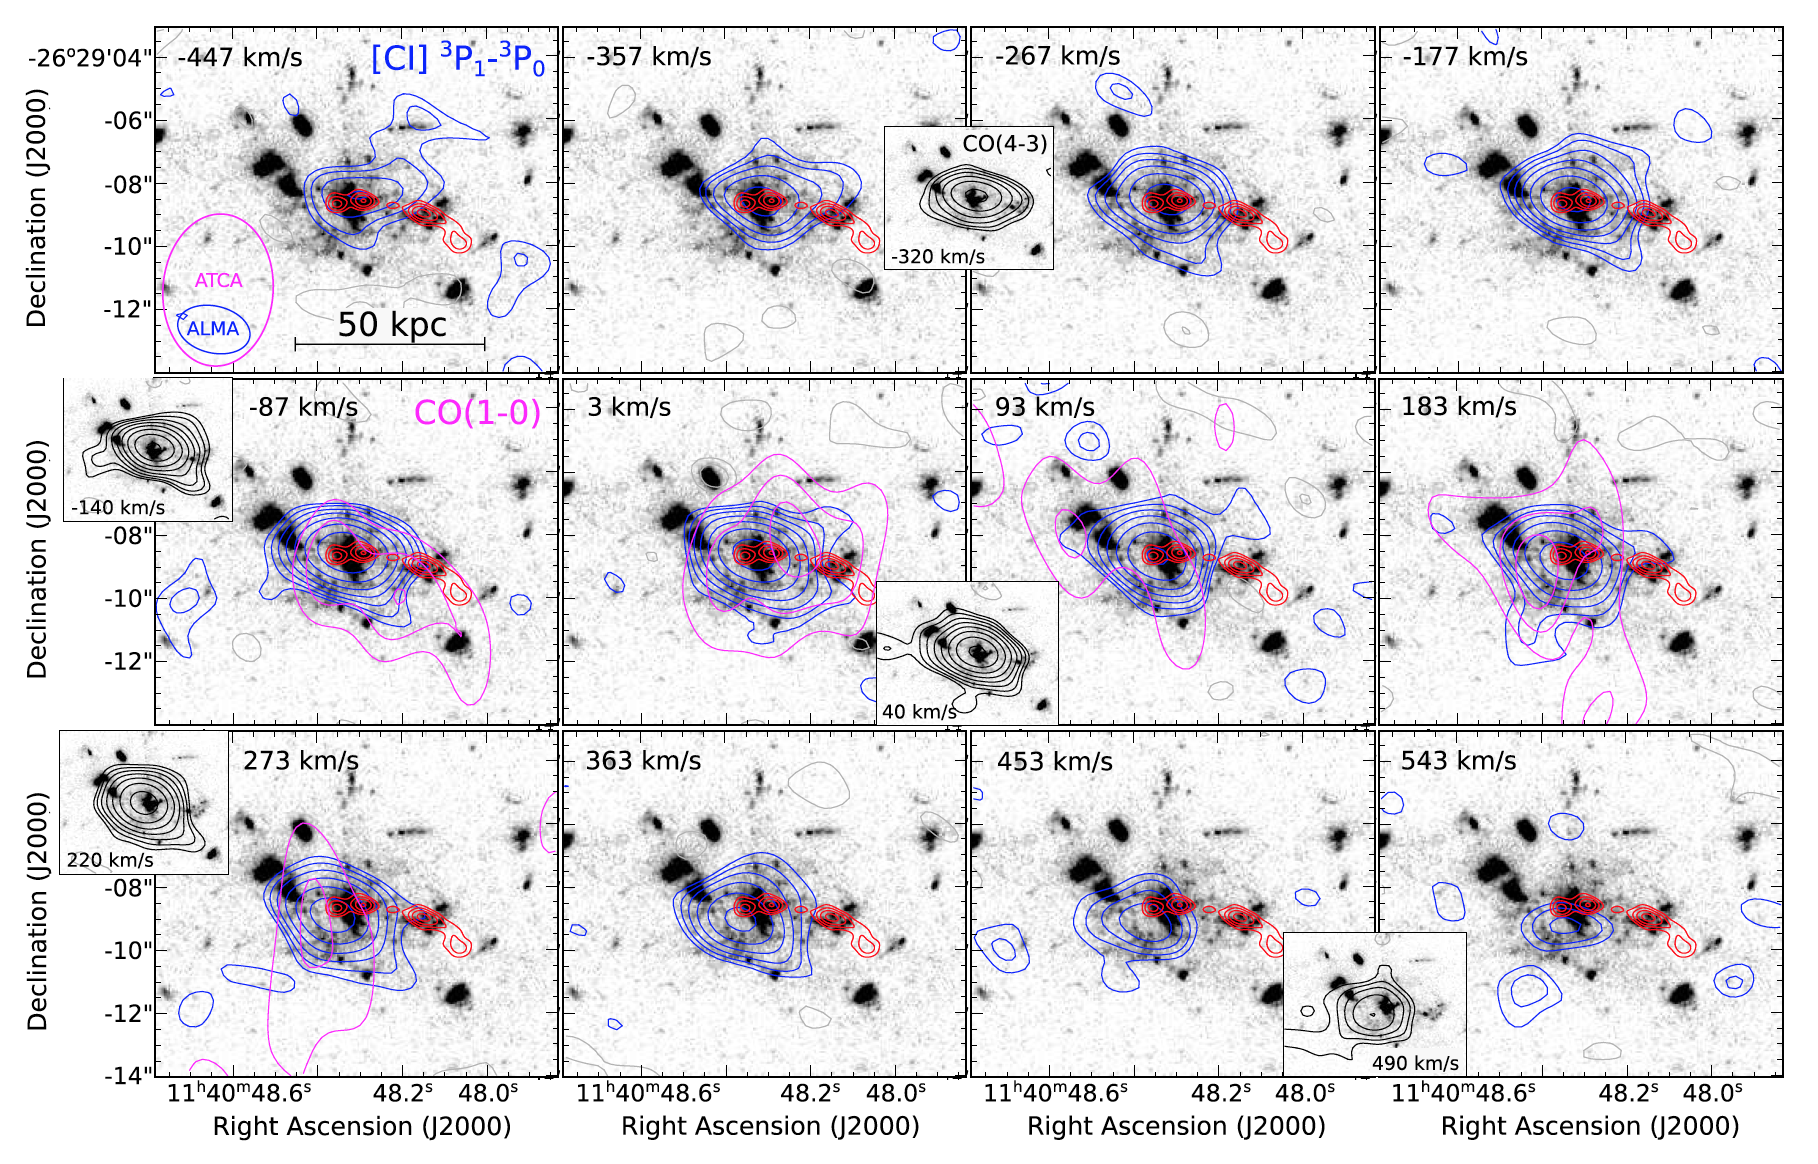
\includegraphics[width=\textwidth]{plots_chp1/Spiderweb_glx_CI_Emonts2018.png}
 \caption[Channels maps of CO(1-0) in MRC1138-262 from \citet{emonts2018}]{Channels maps of the [CI]$^3$P$_1-^3$P$_0$ emission (blue contours) overplotted over an HST/ACS F475W+F814W image from \citet{Miley2006}. The magenta contours indicate the previously detected CO(1-0) emission and the insets show prominent features detected at other velocity channels. Contour levels of [CI] and CO(4-3) start at $2\sigma$ and increase by a factor of 1.5, with $\rm \sigma=0.07~mJy~beam^{-1}$ (negative contours are shown in grey). CO(1-0) contour levels are at $2\sigma,$ $3\sigma,$ $4\sigma,$ $5\sigma$ for $\rm \sigma=0.086~mJy~beam^{-1}.$ The red contours indicate the 36 GHz radio continuum from \citet{Emonts2016}.}
 \label{fig:CI-Spiderweb-Emonts2018}
\end{figure}

Observations in the optical, infrared, mm/sub-mm have provided a substantial proportion of evidence showing that the gaseous nebulae of HzRGs are extended up to distances of $d \lesssim 200$ kpc. Warm, ionised gas tracers have revealed turbulent inner haloes where the radio jets are likely to play a role in driving gas kinematics as well as more quiescent extended gas on the outskirts of the haloes. Is it the radio jets alone that drive the extreme kinematics? The neutral gas traced by absorption in the resonant line Ly$\alpha$ reveals what may be absorption from the Ly$\alpha$ forest or neutral reservoirs of gas within the CGMs of HzRGs. How does the neutral gas find its way into the CGM - is it accreted along filaments from the IGM? If so how may we observe this? The molecular gas component, H$_2,$ traced by CO and [CI] lines show that H$_2$ clouds are frequently observed to preside at projected distances that place them outside the ISMs of HzRGs. Why is H$_2$ rarely traced within the ISM? 

In order to answer questions concerning the kinematics, chemical and morphological structure of the CGMs of distant radio galaxies, deeper observations of sources that have been studied in some detail already, are required. The CGM maintains the imprints of baryon flows and is therefore a kind of forensic tracer for how a given galaxy has emerged to its observed state. Coupling the observations with the results of resolved simulations matched in distance scales will provide better insight into determining the mechanisms that operate over Myr and Gyr time-scales that control the thermodynamic, ionisation state of baryons gravitationally bound to the extended gas halo of a galaxy.

\newpage
\bibliographystyle{mnras}
\bibliography{intro_1_3}


\end{document}